\chapter{Mesh Data Structures}\label{ch:ds}

The algorithms of the following chapters do not only read vertex positions: they walk around
vertices, visit the neighbours of a face, find boundary loops, and modify the connectivity by
splitting, collapsing and flipping edges. The data structure that stores a mesh determines how
fast these operations are and how much memory they need. This chapter compares the classical
choices, from the simplest list of triangles to the half-edge structure used by most geometry
processing libraries.

\section{Requirements}

A mesh data structure must answer three kinds of requests efficiently:
\begin{enumerate}
  \item \textbf{Rendering and geometric queries}: positions of the vertices of a face, normals,
  areas, bounding boxes.
  \item \textbf{Adjacency queries}: the vertices, edges and faces incident to a vertex (its
  \emph{one-ring}), the faces adjacent to a face, the two faces of an edge, whether an element lies
  on the boundary.
  \item \textbf{Modifications}: inserting and deleting elements, splitting faces and edges,
  collapsing edges and flipping them (\cref{ch:ops,ch:remesh}).
\end{enumerate}
We measure memory per vertex using the ratios of \cref{ch:repr}: $F\approx 2V$ and $E\approx 3V$,
4 bytes per index and 12 bytes per position (three single-precision floats).

\section{Face-based structures}

\paragraph{Face set.} The simplest structure stores, for each triangle, the three positions of its
corners. This is the STL format used by 3D printers. It needs $3\times12=36$ bytes per face, that
is $72$ bytes per vertex, and it stores every position about six times. There is no explicit
connectivity: two triangles are neighbours only if they happen to share coordinates, so
adjacency queries require comparing floating-point positions, which is slow and fragile.

\paragraph{Indexed face set.} Vertices are stored once in an array and each face stores three
indices into it. This is the structure of the OBJ, OFF and PLY formats and of most rendering APIs
(vertex and index buffers). Memory is $12$ bytes per vertex plus $12$ bytes per face, about $36$
bytes per vertex. For example, a tetrahedron in OFF format is
\begin{lstlisting}[language={},numbers=none]
OFF
4 4 0
0 0 0
1 0 0
0 1 0
0 0 1
3 0 2 1
3 0 1 3
3 0 3 2
3 1 2 3
\end{lstlisting}
where each face lists its vertices counter-clockwise when seen from outside, so the normal
$(\bx_b-\bx_a)\times(\bx_c-\bx_a)$ points outwards. The indexed face set shares vertices, which
makes the mesh topologically meaningful, but adjacency queries remain expensive: finding the faces
around a vertex requires scanning all faces, $O(F)$ per query.

\paragraph{Face-based connectivity.} Adding references makes local queries constant time. Each
face stores its three vertices and its three neighbouring faces, and each vertex stores one
incident face. This needs $16$ bytes per vertex and $24$ bytes per face, about $64$ bytes per
vertex. Walking around a vertex is possible (from a face, move to the neighbour that shares the
vertex) but requires case distinctions to know which of the three neighbours to take, and the
structure only supports triangles (or a fixed polygon size).

\section{Edge-based structures}

\paragraph{Winged edge.} The winged-edge structure of \citet{Baumgart1975} is built around
edges. Each edge stores its two vertices, its two faces, and the previous and next edges in each of
the two faces (the four ``wings''): 8 references, 32 bytes. Each vertex and face stores one
incident edge. Memory is about $120$ bytes per vertex, and since an edge has no intrinsic
orientation, every traversal step must test in which of the two faces it is moving.

\paragraph{Half-edge.} The half-edge structure \citep{Mantyla1988,Kettner1999} removes the
orientation ambiguity by splitting each edge into two directed \emph{half-edges} with opposite
directions. Each half-edge belongs to exactly one face, which it traverses counter-clockwise, and
stores (\cref{fig:halfedge}):
\begin{itemize}
  \item the vertex it points to, $\operatorname{to}(h)$;
  \item its opposite half-edge, $\operatorname{opp}(h)$;
  \item the next half-edge in its face, $\operatorname{next}(h)$ (optionally also
  $\operatorname{prev}(h)$);
  \item its face, $\operatorname{face}(h)$, or a null value for boundary half-edges.
\end{itemize}
Each vertex stores one outgoing half-edge and each face one of its half-edges. With $6V$
half-edges of 16 bytes (20 with $\operatorname{prev}$), memory is about $120$ to $144$ bytes per
vertex. All adjacency queries become short loops without case distinctions, the structure handles
arbitrary polygons, and boundaries are represented by half-edges without a face.

\begin{figure}[tbp]
\centering
\begin{tikzpicture}[scale=1.25, every node/.style={font=\small},
  he/.style={-{Stealth[length=2.2mm]}, thick}, op/.style={-{Stealth[length=2.2mm]}, thick, BrickRed}]
  \coordinate (A) at (0,0); \coordinate (B) at (3,0); \coordinate (C) at (1.5,2.1); \coordinate (D) at (1.5,-2.1);
  \fill[MidnightBlue!6] (A) -- (B) -- (C) -- cycle;
  \fill[black!4] (A) -- (D) -- (B) -- cycle;
  \draw (A) -- (B) -- (C) -- cycle; \draw (A) -- (D) -- (B);
  \foreach \p in {A,B,C,D} \fill (\p) circle (1.6pt);
  % half-edges of the upper face (counter-clockwise)
  \draw[he, MidnightBlue] ($(A)!0.12!(B)+(0,0.1)$) -- ($(A)!0.88!(B)+(0,0.1)$) node[midway, above] {$h$};
  \draw[he] ($(B)!0.14!(C)+(-0.09,-0.03)$) -- ($(B)!0.86!(C)+(-0.09,-0.03)$) node[midway, right=2pt] {$\operatorname{next}(h)$};
  \draw[he] ($(C)!0.14!(A)+(0.09,-0.03)$) -- ($(C)!0.86!(A)+(0.09,-0.03)$) node[midway, left=2pt] {$\operatorname{prev}(h)$};
  \draw[op] ($(B)!0.12!(A)+(0,-0.1)$) -- ($(B)!0.88!(A)+(0,-0.1)$) node[midway, below] {$\operatorname{opp}(h)$};
  \node at (1.5,0.75) {$\operatorname{face}(h)$};
  \node[below left] at (A) {$\operatorname{from}(h)$};
  \node[below right] at (B) {$\operatorname{to}(h)$};
\end{tikzpicture}
\caption{The half-edge $h$ goes from vertex $\operatorname{from}(h)$ to $\operatorname{to}(h)$ and
belongs to the face on its left. Its successor and predecessor in that face are
$\operatorname{next}(h)$ and $\operatorname{prev}(h)$; the half-edge running in the opposite
direction, in the neighbouring face, is $\operatorname{opp}(h)$.}
\label{fig:halfedge}
\end{figure}

\subsection{Traversals}

The defining operation of the half-edge structure is the circulation around a vertex. Starting
from an outgoing half-edge $h$ of vertex $v$, the next outgoing half-edge in counter-clockwise
order is $\operatorname{opp}(\operatorname{prev}(h))$, and in clockwise order
$\operatorname{next}(\operatorname{opp}(h))$. \Cref{alg:onering} lists the one-ring; the same loop
gives the incident faces ($\operatorname{face}(h)$) and the valence (number of iterations).

\begin{algorithm}[tbp]
\caption{One-ring of a vertex in a half-edge mesh.}\label{alg:onering}
\Input{vertex $v$ with outgoing half-edge $h_0=\operatorname{out}(v)$}
\Output{list $R$ of neighbouring vertices in counter-clockwise order}
$R\gets[\,]$; $h\gets h_0$\;
\Repeat{$h=h_0$}{
  append $\operatorname{to}(h)$ to $R$\;
  $h\gets\operatorname{opp}(\operatorname{prev}(h))$\tcp*{rotate to the next outgoing half-edge}
}
\end{algorithm}

Other queries are equally local. The two faces of an edge are $\operatorname{face}(h)$ and
$\operatorname{face}(\operatorname{opp}(h))$; the vertices of a face are obtained by following
$\operatorname{next}$ until returning to the start; a vertex is on the boundary if one of its
outgoing half-edges has no face, and conventionally $\operatorname{out}(v)$ is chosen to be that
half-edge, so the test is $O(1)$; boundary loops are traced by following $\operatorname{next}$
among boundary half-edges.

\fig[0.95\textwidth]{ch03_halfedge_valence.png}{Left: circulation around a vertex with the
rule $h\leftarrow\operatorname{opp}(\operatorname{prev}(h))$; the numbers give the visiting order of
the outgoing half-edges. Right: valence histograms of the bunny (mean $5.99$) and the armadillo
(mean $6.00$), as predicted by Euler's formula.}{fig:valence}

\subsection{Building a half-edge mesh from an indexed face set}

\begin{enumerate}
  \item For every face $(a,b,c)$ create the half-edges $a\to b$, $b\to c$, $c\to a$ with their
  $\operatorname{next}$ links and face, and insert each one in a hash map keyed by the ordered pair
  $(\text{from},\text{to})$.
  \item For every half-edge $i\to j$, look up $(j,i)$; if found, link them as opposites.
  \item Half-edges without opposite are on the boundary: create the missing boundary half-edges
  (without face) and link them into boundary loops.
  \item If a key $(i,j)$ appears twice, two faces traverse the same edge in the same direction: the
  mesh is either inconsistently oriented or non-manifold, and must be repaired first.
\end{enumerate}
The construction is $O(F)$ expected time. The same pairing step is how orientation consistency is
checked in practice.

\begin{example}{Two triangles}{twotri}
Take faces $f_0=(0,1,2)$ and $f_1=(0,2,3)$, a square split along the diagonal $0$--$2$. The
half-edges of $f_0$ are $h_0:0\to1$, $h_1:1\to2$, $h_2:2\to0$ and those of $f_1$ are $h_3:0\to2$,
$h_4:2\to3$, $h_5:3\to0$. The only pair of opposite keys is $(2,0)$ and $(0,2)$, so
$\operatorname{opp}(h_2)=h_3$. The other four half-edges are on the boundary and get boundary
partners. Circulating around vertex $0$ from $h_0$: $\operatorname{prev}(h_0)=h_2$, so the next
outgoing half-edge is $\operatorname{opp}(h_2)=h_3$; then $\operatorname{prev}(h_3)=h_5$, whose
opposite is the boundary half-edge $0\to3$, which closes the loop. The one-ring of $0$ is
$(1,2,3)$, in counter-clockwise order.
\end{example}

\section{Index-based structures for triangle meshes}

For pure triangle meshes the half-edges can be numbered implicitly, so that most pointers are
computed instead of stored.

\paragraph{Directed edges.} \citet{Campagna1998} number the half-edges of face $f$ as $3f$,
$3f+1$, $3f+2$. Then
\begin{equation}
\operatorname{face}(h)=\lfloor h/3\rfloor,\qquad
\operatorname{next}(h)=3\lfloor h/3\rfloor+(h+1)\bmod 3,\qquad
\operatorname{prev}(h)=3\lfloor h/3\rfloor+(h+2)\bmod 3,
\end{equation}
and only $\operatorname{to}(h)$ (which is the face's index array) and $\operatorname{opp}(h)$ are
stored. Memory drops to about $64$ bytes per vertex while keeping all half-edge traversals.

\paragraph{Corner table.} \citet{Rossignac2001} use the same idea with \emph{corners}: corner
$c=3f+i$ is the $i$-th corner of face $f$, $V[c]$ is its vertex and $O[c]$ the opposite corner
across the edge facing $c$. The next and previous corners are computed arithmetically. The corner
table was designed for mesh compression (Edgebreaker) and is used by GPU-friendly libraries.

\paragraph{Beyond manifold surfaces.} Half-edges cannot represent an edge with three faces or a
vertex with two fans. Non-manifold models (for example CAD assemblies or meshes produced by
Boolean operations) need dedicated structures \citep{DeFloriani2003}, or a preprocessing step that
splits non-manifold vertices and edges. Compact array-based variants of the half-edge idea also exist
for volumetric meshes \citep{Lage2005}.

\begin{table}[tbp]
\centering\small
\begin{tabular}{@{}lccc@{}}
\toprule
Structure & Bytes per vertex & One-ring query & Arbitrary polygons \\
\midrule
Face set (STL) & 72 & no connectivity & yes \\
Indexed face set (OBJ/OFF) & 36 & $O(F)$ & yes \\
Face-based connectivity & 64 & $O(1)$, case analysis & no \\
Winged edge & 120 & $O(1)$, case analysis & yes \\
Half-edge & 120--144 & $O(1)$ per step & yes \\
Directed edges / corner table & 64 & $O(1)$ per step & triangles only \\
\bottomrule
\end{tabular}
\caption{Memory and adjacency support of mesh data structures (4-byte indices, 12-byte
positions, $F\approx2V$, $E\approx3V$).}
\label{tab:ds}
\end{table}

\section{Modifying the connectivity}

Local modifications are expressed as small rewirings of the half-edge pointers. The three
operations used by simplification and remeshing are (\cref{fig:edgeops}):
\begin{itemize}
  \item \textbf{Edge split}: insert a vertex in the middle of an edge and connect it to the
  opposite vertices of the two adjacent triangles ($+1$ vertex, $+3$ edges, $+2$ faces).
  \item \textbf{Edge collapse}: merge the two endpoints of an edge into one vertex, removing the
  edge and its two adjacent triangles ($-1$ vertex, $-3$ edges, $-2$ faces).
  \item \textbf{Edge flip}: replace the diagonal of the quadrilateral formed by two adjacent
  triangles by the other diagonal (the counts do not change).
\end{itemize}
All three preserve the Euler characteristic, as they must. They are \emph{Euler operators}
\citep{Mantyla1988}: by composing them, any manifold triangulation of a given topology can be
transformed into any other. An edge collapse is only legal if it does not change the topology: the
\emph{link condition} requires that the endpoints $p,q$ share exactly two common neighbours (the
opposite vertices of the two triangles), otherwise the collapse would create a non-manifold edge.

\begin{figure}[tbp]
\centering
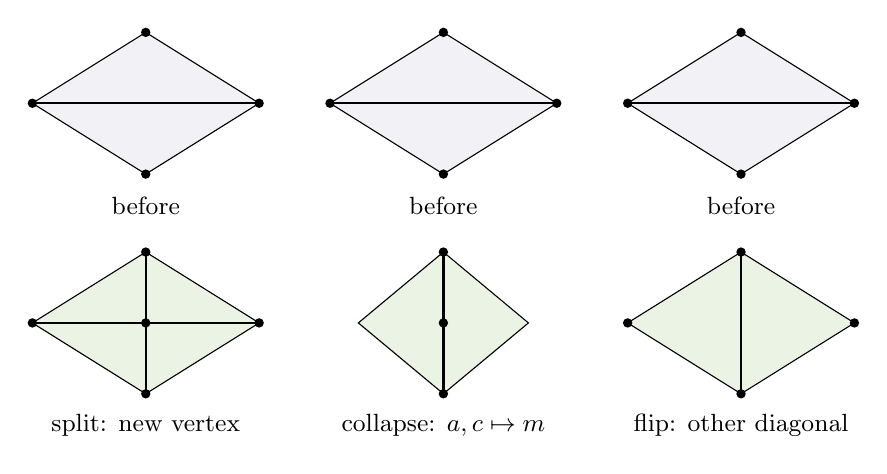
\begin{tikzpicture}[scale=0.9, every node/.style={font=\small}]
  \tikzset{v/.style={circle, fill, inner sep=1.2pt}}
  \foreach \dx/\name in {0/split, 4.2/collapse, 8.4/flip} {
    \begin{scope}[xshift=\dx cm]
      \coordinate (a) at (0,0); \coordinate (b) at (1.6,1); \coordinate (c) at (3.2,0); \coordinate (d) at (1.6,-1);
      \draw[fill=MidnightBlue!6] (a) -- (b) -- (c) -- (d) -- cycle;
      \draw[thick] (a) -- (c);
      \foreach \p in {a,b,c,d} \node[v] at (\p) {};
      \node at (1.6,-1.45) {before};
    \end{scope}
  }
  % after states drawn below
  \begin{scope}[yshift=-3.1cm]
    \coordinate (a) at (0,0); \coordinate (b) at (1.6,1); \coordinate (c) at (3.2,0); \coordinate (d) at (1.6,-1); \coordinate (m) at (1.6,0);
    \draw[fill=OliveGreen!8] (a) -- (b) -- (c) -- (d) -- cycle; \draw[thick] (a) -- (c); \draw[thick] (b) -- (d);
    \foreach \p in {a,b,c,d,m} \node[v] at (\p) {};
    \node at (1.6,-1.45) {split: new vertex};
  \end{scope}
  \begin{scope}[xshift=4.2cm, yshift=-3.1cm]
    \coordinate (b) at (1.6,1); \coordinate (m) at (1.6,0); \coordinate (d) at (1.6,-1);
    \draw[fill=OliveGreen!8] (0.4,0) -- (b) -- (2.8,0) -- (d) -- cycle;
    \draw[thick] (b) -- (m) -- (d);
    \foreach \p in {b,m,d} \node[v] at (\p) {};
    \node at (1.6,-1.45) {collapse: $a,c\mapsto m$};
  \end{scope}
  \begin{scope}[xshift=8.4cm, yshift=-3.1cm]
    \coordinate (a) at (0,0); \coordinate (b) at (1.6,1); \coordinate (c) at (3.2,0); \coordinate (d) at (1.6,-1);
    \draw[fill=OliveGreen!8] (a) -- (b) -- (c) -- (d) -- cycle; \draw[thick] (b) -- (d);
    \foreach \p in {a,b,c,d} \node[v] at (\p) {};
    \node at (1.6,-1.45) {flip: other diagonal};
  \end{scope}
\end{tikzpicture}
\caption{The three local connectivity operations on the edge $(a,c)$ shared by two triangles. In
a full mesh the collapse also reconnects all the other neighbours of $a$ and $c$ to the merged
vertex $m$.}
\label{fig:edgeops}
\end{figure}

\begin{keypoints}
\begin{itemize}[leftmargin=*]
  \item Indexed face sets are compact and universal for storage and rendering, but adjacency
  queries cost $O(F)$.
  \item The half-edge structure gives constant-time local traversals without case distinctions,
  at about $120$--$144$ bytes per vertex; the one-ring is visited with
  $h\leftarrow\operatorname{opp}(\operatorname{prev}(h))$.
  \item For triangle meshes, directed edges and corner tables compute most pointers
  arithmetically and halve the memory.
  \item Split, collapse and flip are the building blocks of simplification and remeshing; collapses
  must satisfy the link condition.
\end{itemize}
\end{keypoints}

\section*{Exercises}
\begin{exercise}
Write the clockwise one-ring traversal and show that it visits the same vertices as
\cref{alg:onering} in reverse order. What changes for a boundary vertex?
\end{exercise}
\begin{exercise}
Using only $\operatorname{to}$, $\operatorname{opp}$ and $\operatorname{next}$ of the directed-edge
structure, write the code that returns the three faces adjacent to face $f$.
\end{exercise}
\begin{exercise}
Show that the link condition is necessary: draw a mesh where collapsing an edge whose endpoints
share three neighbours produces a non-manifold configuration.
\end{exercise}
